%Please use LuaLaTeX or XeLaTeX
\documentclass[11pt,aspectratio=169,reqno]{beamer}

\usepackage[labelformat=empty]{caption}
\usepackage{mhchem}

\title{Titel muss noch erfunden werden}
\date[28.03.2023]{28.03.2023}
\author{Mario Kunz, Xaver Hanushevsky}
\institute{D-BIOL}

\usetheme{eth}

\colorlet{titlefgcolor}{ETHBlue}
\colorlet{accentcolor}{ETHRed}

\newcommand{\highlightpause}{\addtocounter{beamerpauses}{-1}\pause\color<+>{ETHPurple}}

\begin{document}

\titleframe

\begin{frame}[fragile]{Intro}
    Etwas Kreatives einfallen lassen für hier
\end{frame}

\begin{frame}{Was ist Rückkopplung...}
Positiv und negative Rückkopplung mit Bild erklären
Erwartungen an unsere Lösungen (Positiv => $\infty$)
\end{frame}

\begin{frame}{Das Lac Operon}
\begin{columns}
    \column{.4\textwidth}

    \begin{itemize}
        \item Positive Regulation durch cAMP\\
        \begin{itemize}
            \item cAMP Synthese inhibiert in Präsenz von \emph{Glucose}
            \item cAMP bindet and CRP
            \item Homodimer bindet vor Promoter an DNA
            \item Interaktion mit $\alpha$-Untereinheit von RNA Pol führt zu Initiation
        \end{itemize}
        \item Negative Regulation durch freies LacI-Protein
        \begin{itemize}
            \item Allolactose inaktiviert LacI \\ $\ce{Lactose $\xrightleftharpoons{LacY}$ Allolactose}$
        \end{itemize}
        \item[$\Rightarrow$] Lac Operon nur exprimiert in Präsenz von Lactose und Abwesenheit von Glucose
    \end{itemize}

    {\tiny cAMP = cyclic AMP, CRP = cAMP receptor protein}
    
    \column{.6\textwidth}
    \begin{figure}
        \centering
        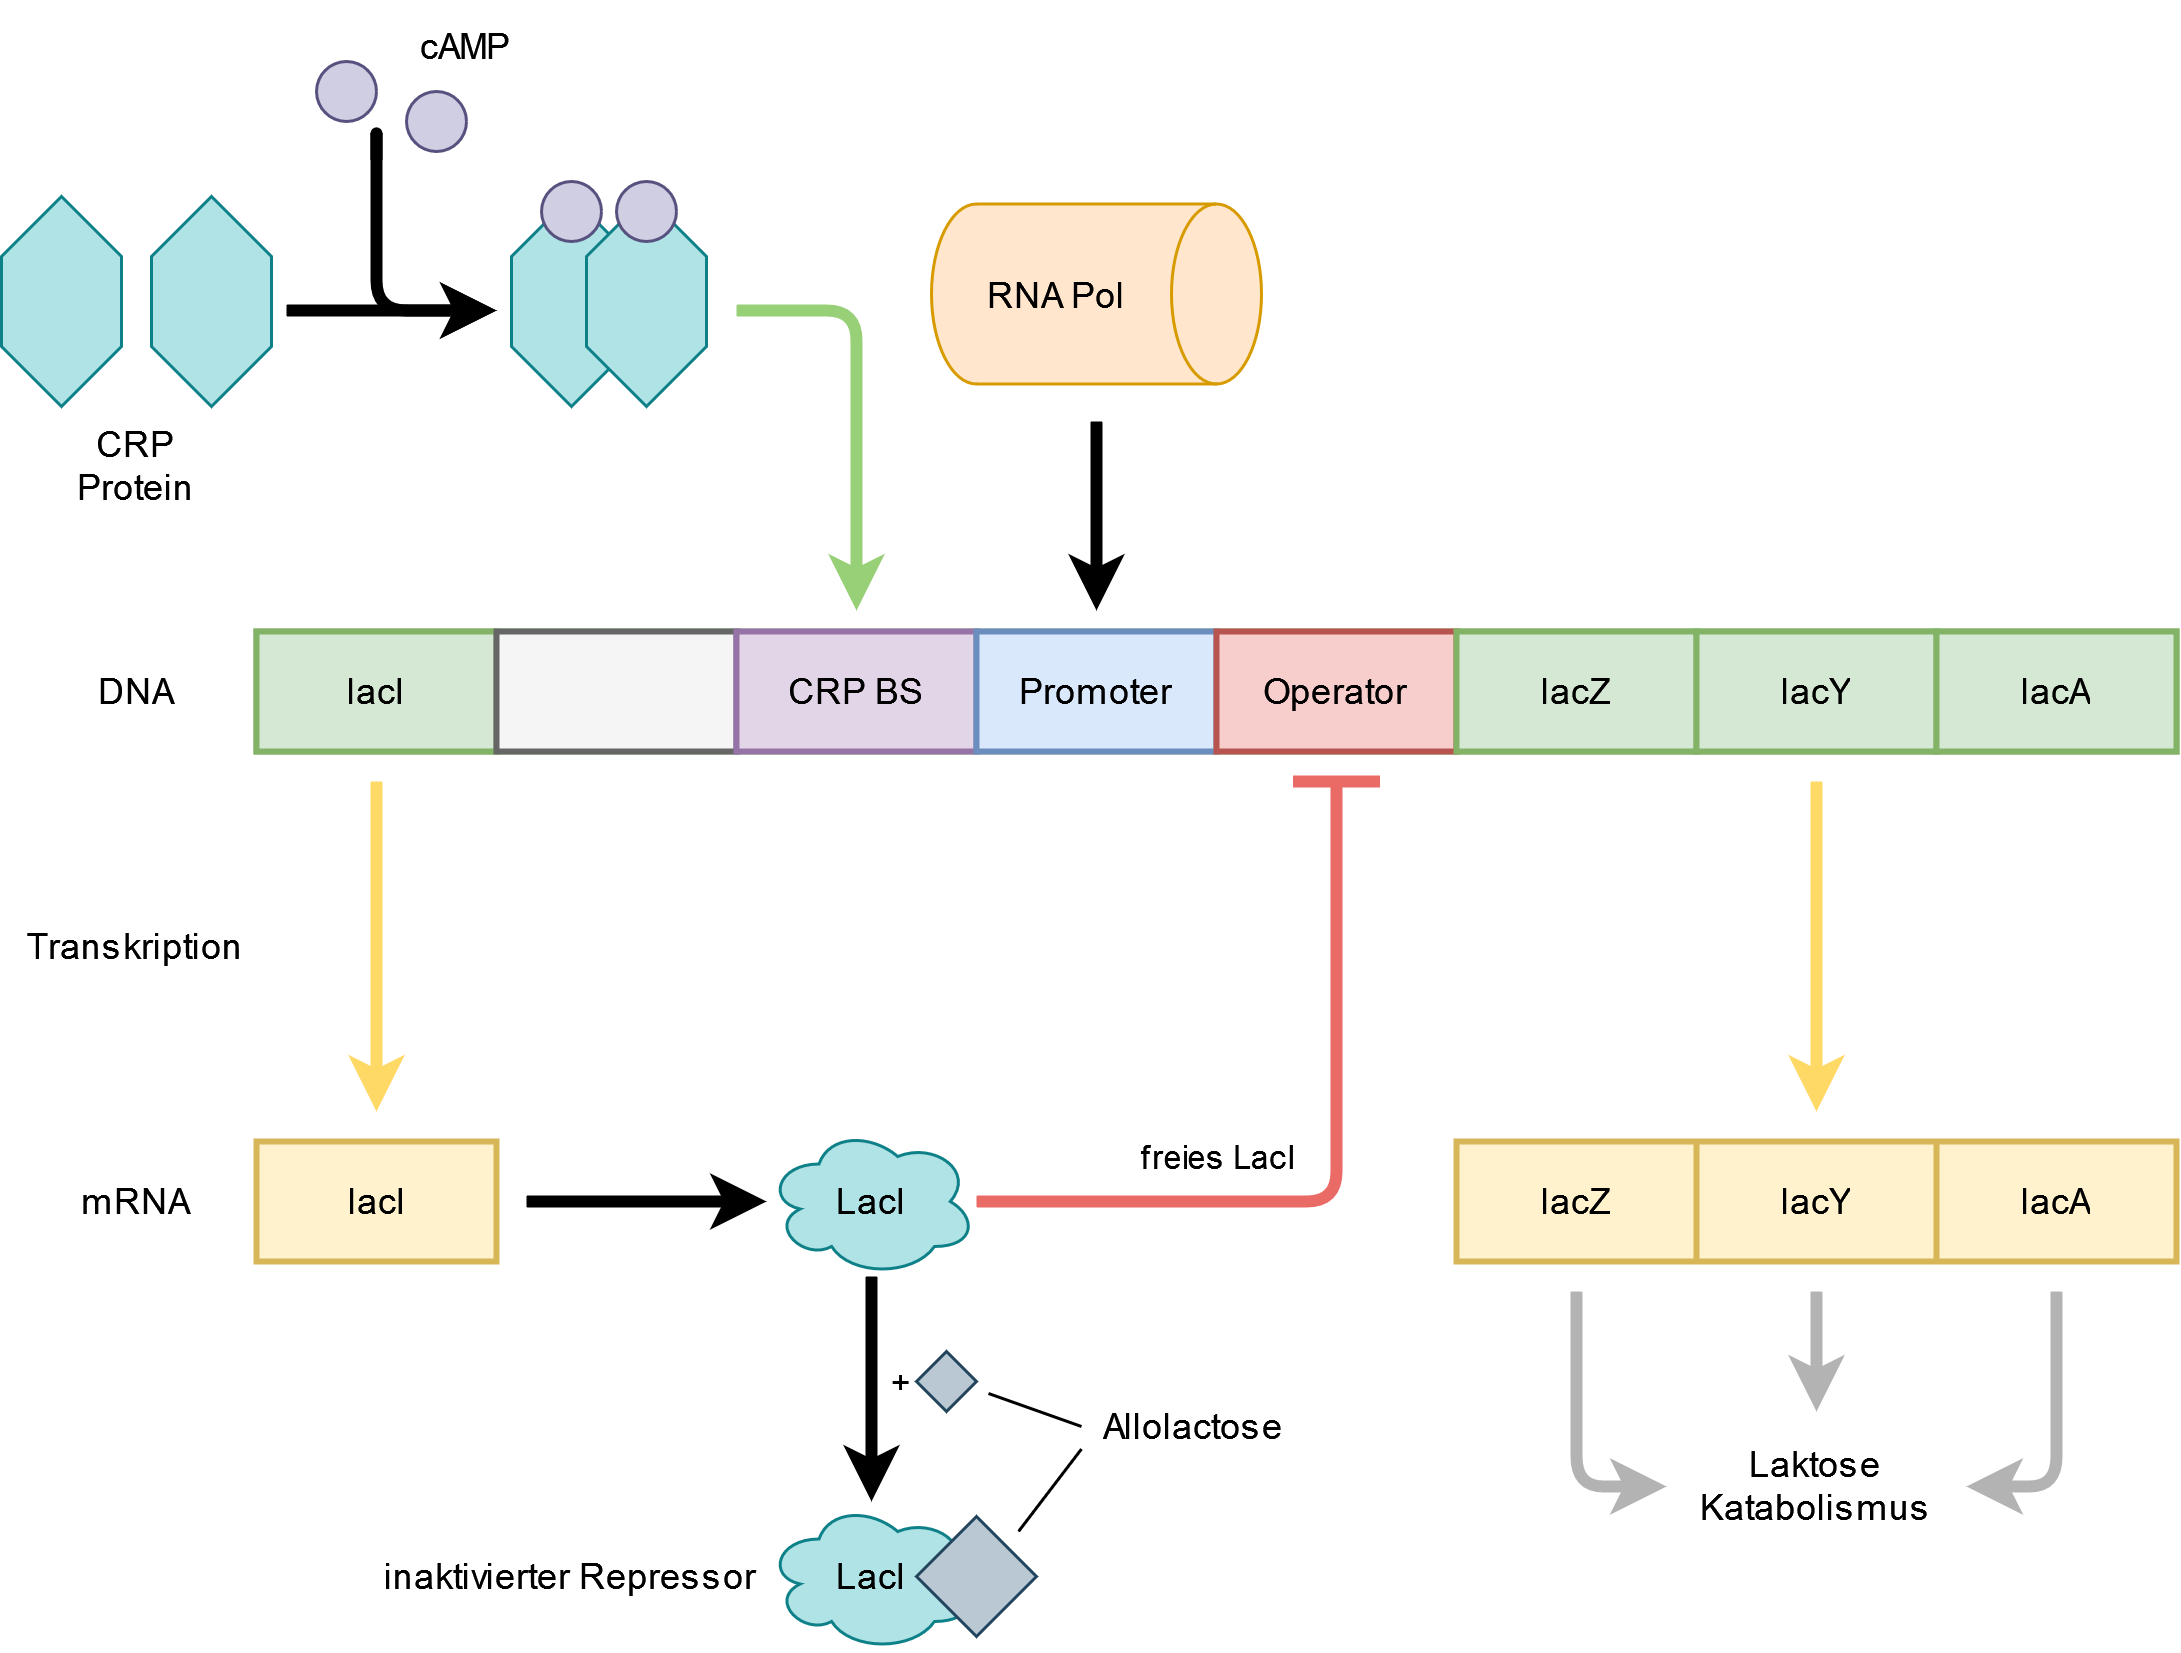
\includegraphics[width=\textwidth]{images/lac_operon.png}
    \end{figure}
\end{columns}
\end{frame}

\begin{frame}{Repression des Lac Operons}
\begin{columns}
    \column{.4\textwidth}

    \begin{itemize}
        \item Repression des lac-operons aus Ausgangspunkt für unser Modell
        \item Überspringen des Abbaus von Lactose/Allolactose
        \item[$\Rightarrow$] Codierte Proteine des Operons binden direkt als Repressor zum Operator
    \end{itemize}
    
    \column{.6\textwidth}
    \begin{figure}
        \centering
        \only<+>{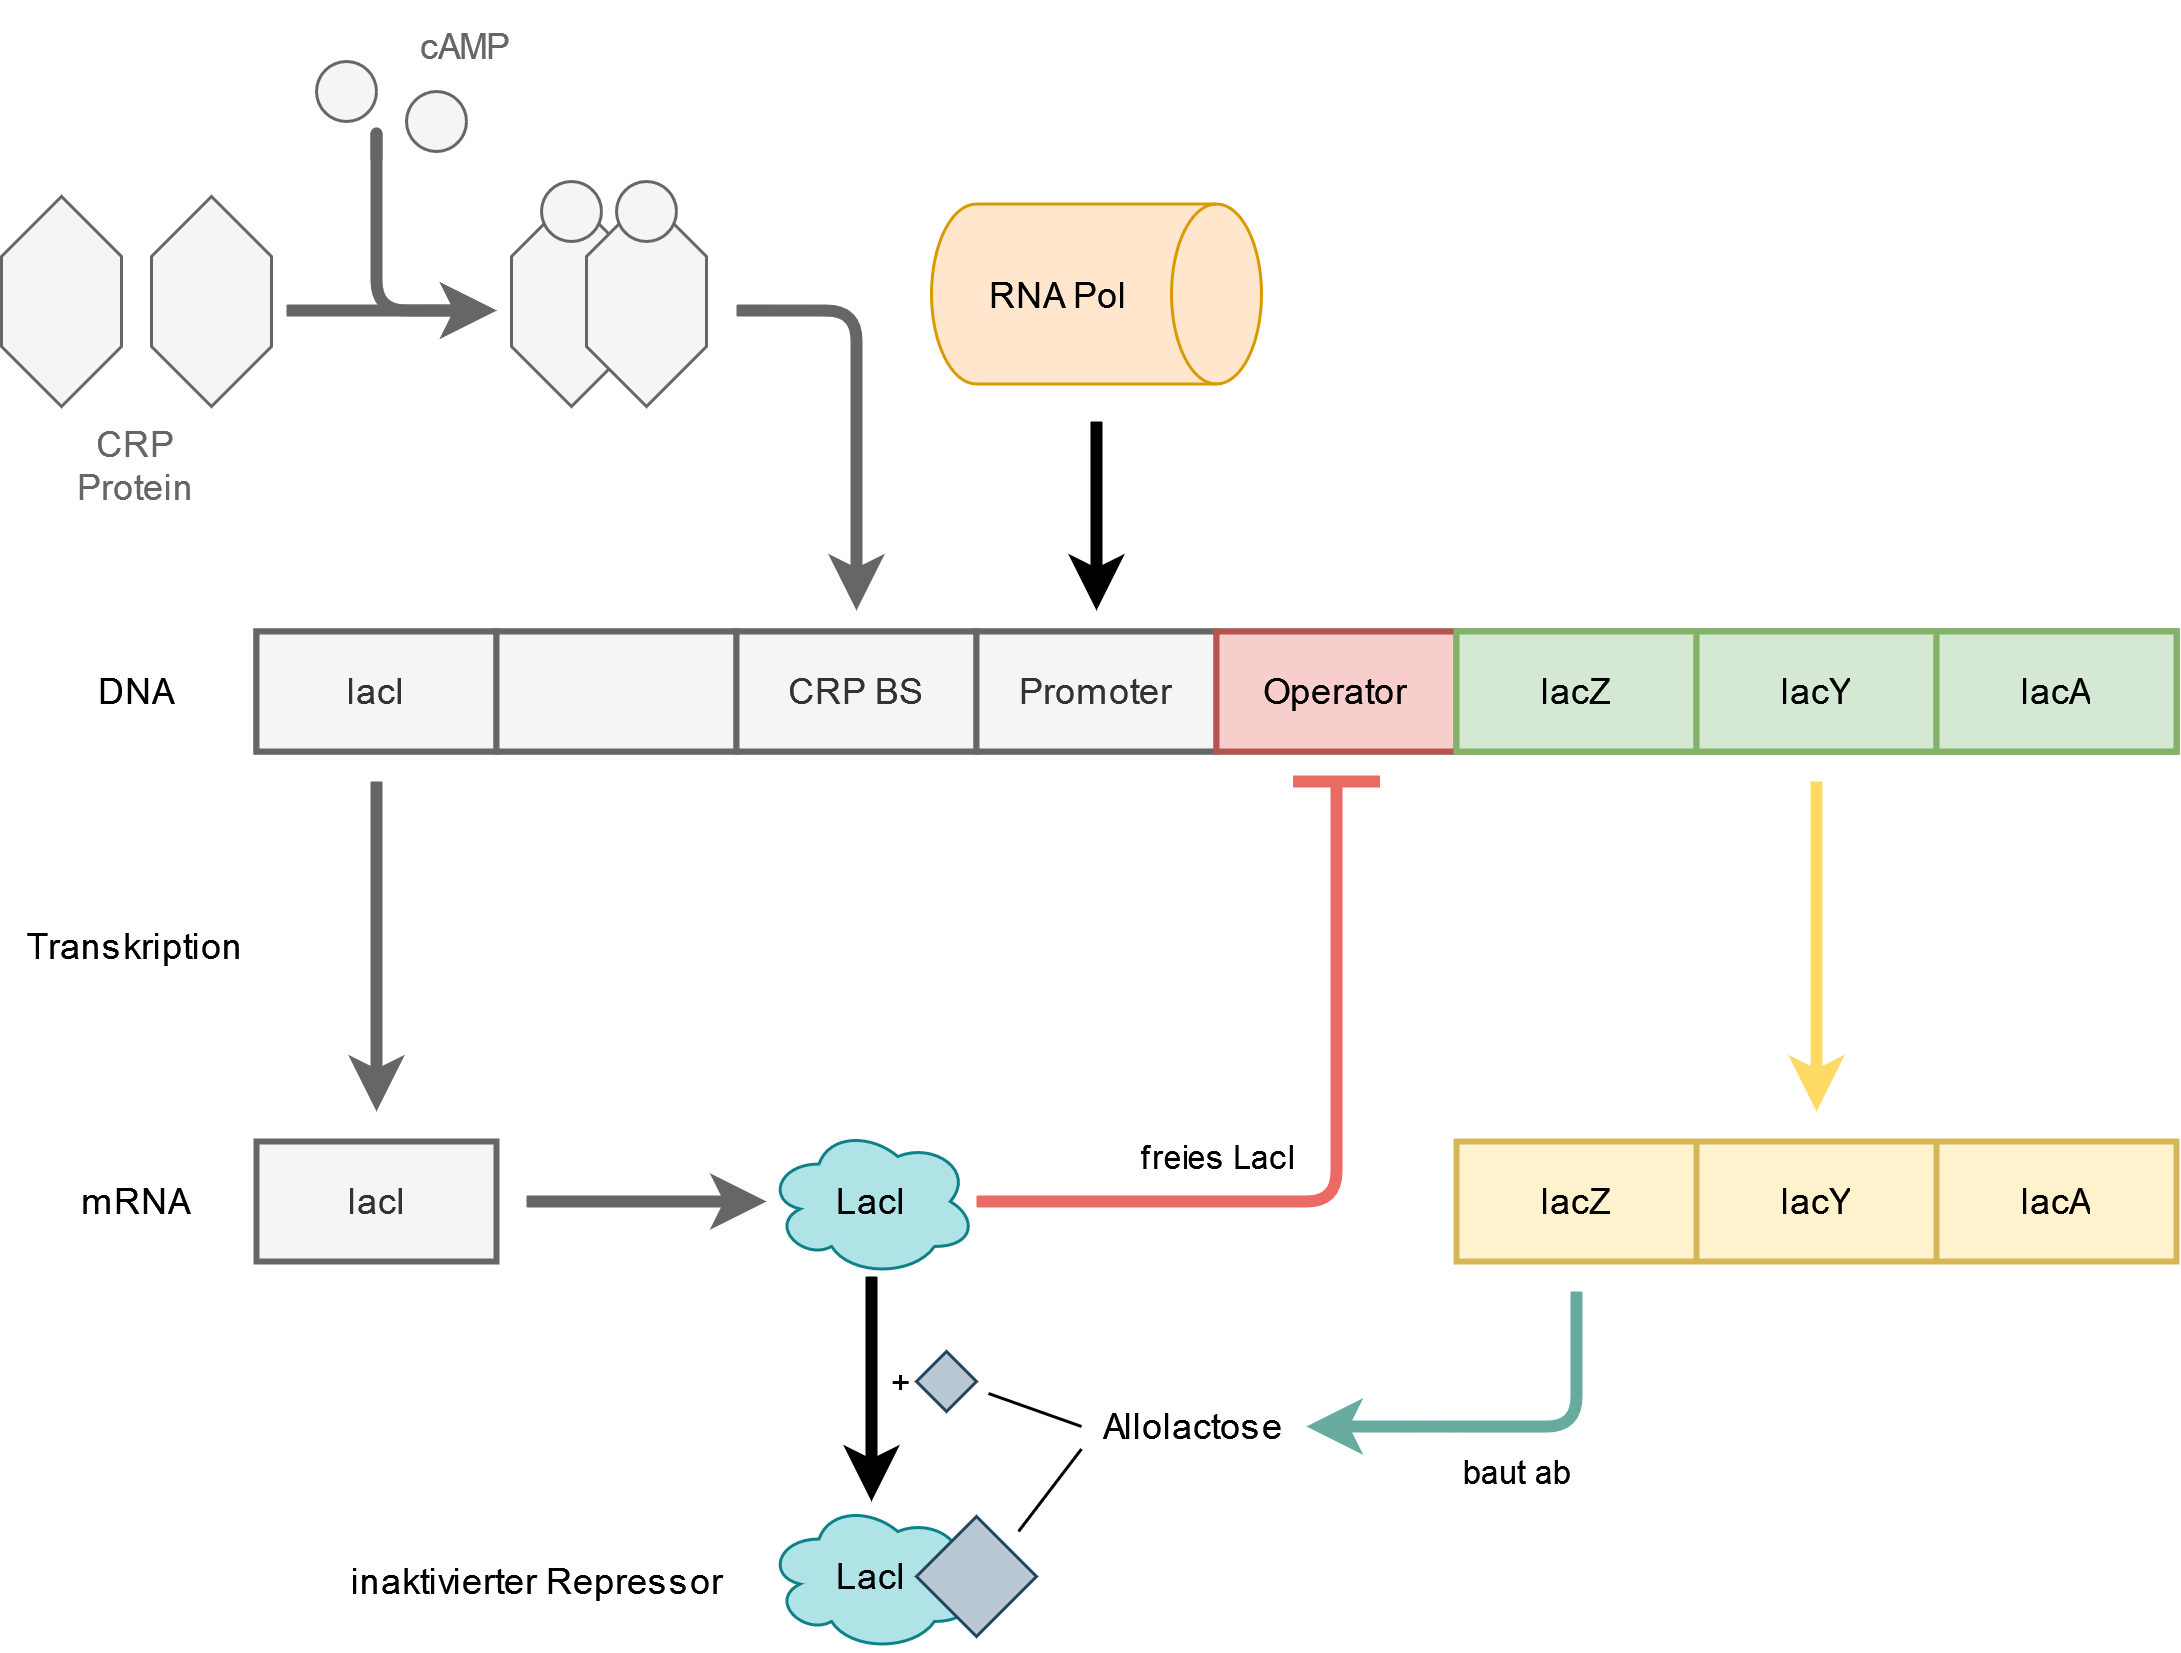
\includegraphics[width=\textwidth]{images/lac_operon_only_repression.png}}
        \only<+>{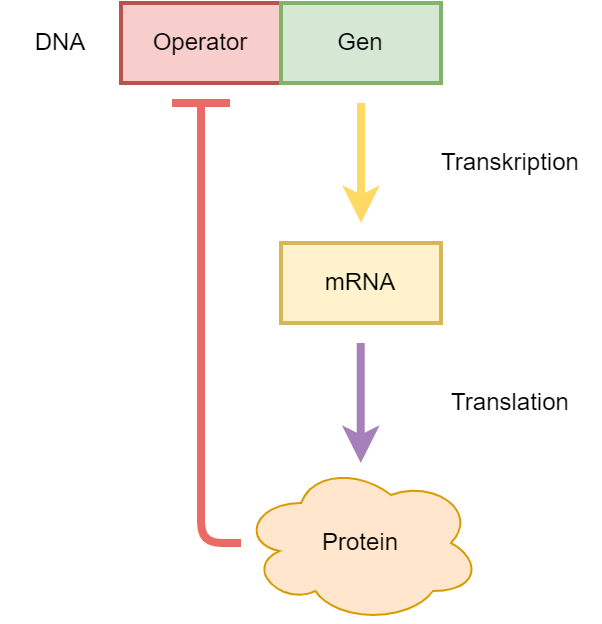
\includegraphics[width=.7\textwidth]{images/repression.png}}
    \end{figure}
\end{columns}
\end{frame}


\begin{frame}{Negative Autoregulation über Repressorprotein}
    \centering Nur freie DNA führt zu Transkription\\ 
    mehr Protein $\Rightarrow$ weniger freie DNA $\Rightarrow$ weniger Transkription

    \begin{figure}
        \centering
        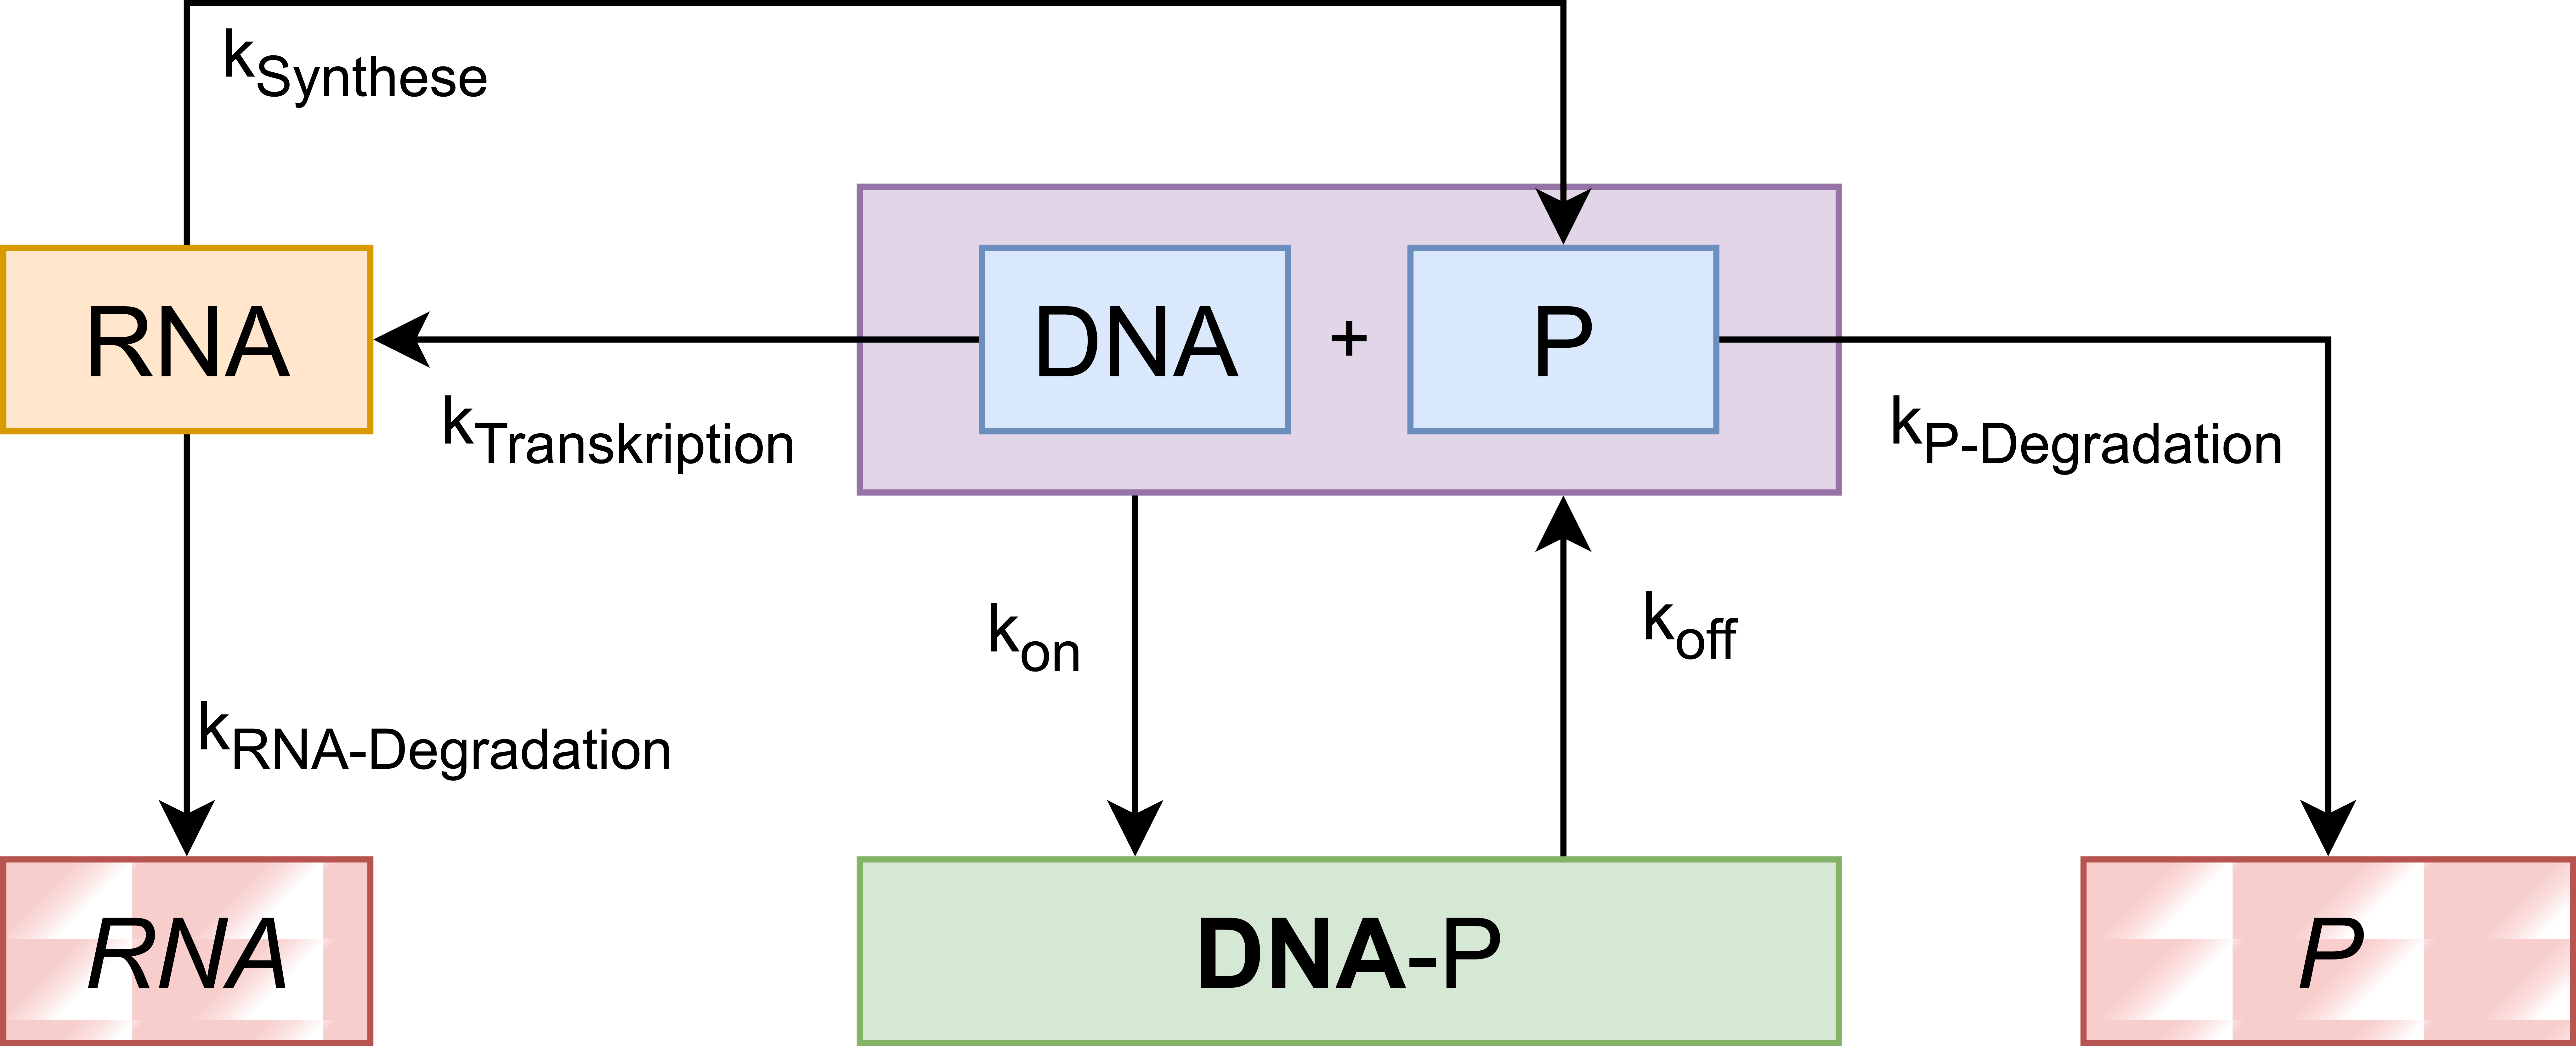
\includegraphics[width=.6\textwidth]{images/negative_autoregulation_overview.png}
    \end{figure}
\end{frame}

\begin{frame}{Gleichgewicht zwischen gebundener und freier DNA}
    \begin{tikzpicture}[remember picture,overlay]
        \node[xshift=-2cm,yshift=-1.5cm] at (current page.north east) {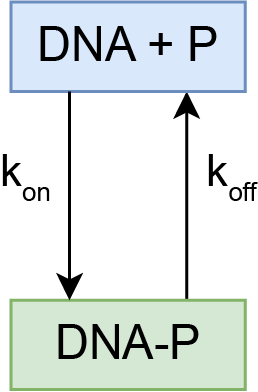
\includegraphics[width=2cm]{images/DNA-binding_equilibrium.png}};
    \end{tikzpicture}

    Hin- und Rückreaktionen im Gleichgewicht
    \begin{itemize}
        \item $v_\text{on}=k_\text{on}\cdot [\text{DNA}]\cdot [\text{P}]$
        \item $v_\text{off}=k_\text{off}\cdot [\text{DNA-P}]$\pause
    \end{itemize}

    \vspace{1.5em}

    \begin{columns}[onlytextwidth]
    \column{.4\textwidth}
    Für die folgenden Schritte nehmen wir an, dass sich das DNA-Protein Gleichgewicht sehr schnell einstellt, denn dann gilt:
    \column{.6\textwidth}
    \begin{itemize}
        \item $v_\text{on}=v_\text{off}$\\[8pt]
        \item $\dfrac{d[\text{DNA}]}{dt}=-\dfrac{d[\text{DNA-P}]}{dt}=0$\\[8pt]
    \end{itemize}
    \[k_\text{on}\cdot [\text{DNA}]\cdot [\text{P}]=k_\text{off}\cdot [\text{DNA-P}]\]
    \end{columns}
\end{frame}

\begin{frame}{Gleichgewicht zwischen gebundener und freier DNA}
    \begin{columns}[T]
    \column{.3\textwidth}
    \centering
    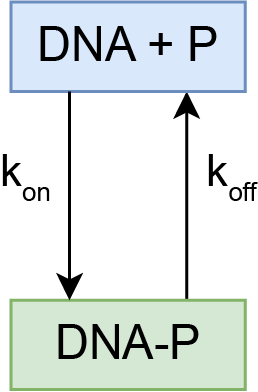
\includegraphics[width=2cm]{images/DNA-binding_equilibrium.png}
    \column{.3\textwidth}
    \[K=\frac{k_\text{off}}{k_\text{on}}=\frac{[\text{DNA}]\cdot [\text{P}]}{[\text{DNA-P}]}\]\pause
    \column{.3\textwidth}
        \[[\text{DNA$_\text{Total}$}]=[\text{DNA}]+[\text{DNA-P}]\]\\[-2em]
        \[[\text{DNA}]=[\text{DNA$_\text{Total}$}]-[\text{DNA-P}]\]
    \end{columns}

    \vspace{4em}
    \highlightpause
    
    \parbox{\textwidth}{
    % \[\Downarrow\]
    % \[K=\frac{([\text{DNA$_\text{Total}$}]-[\text{DNA-P}])\cdot [\text{P}]}{[\text{DNA-P}]}\]\\
    % \[K\cdot[\text{DNA-P}]=[\text{DNA$_\text{Total}$}]\cdot [\text{P}]-[\text{DNA-P}]\cdot [\text{P}]\]
    % \[[\text{DNA-P}]\cdot(K+[\text{P}])=[\text{DNA$_\text{Total}$}]\cdot [\text{P}]\]\\
    \[[\text{DNA-P}]=\frac{[\text{DNA$_\text{Total}$}]\cdot [\text{P}]}{K+[\text{P}]}\]
    }
\end{frame}

\begin{frame}{Vergleich mit Bindungsgleichgewichte, Grundlagen der Biologie 1}
    \begin{columns}
        \column{.4\textwidth}
        Konzentration der besetzten DNA\vspace{1em}
        \[[\text{DNA-P}]=[\text{DNA$_\text{Total}$}]\cdot\color{ETHPurple}\frac{[\text{P}]}{K+[\text{P}]}\]
        \pause
        
        \column{.6\textwidth}
        \begin{figure}
            \centering
            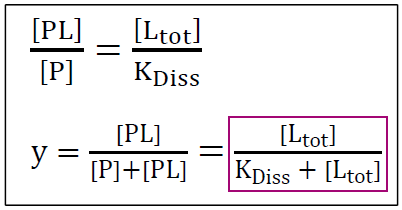
\includegraphics[width=.6\textwidth]{images/occuption_degree_glockshuber.png}
            \caption*{\tiny Skript Prof. Dr. Rudolf Glockshuber, S. 32}
        \end{figure}
        
        \begin{description}
            \item[$K_\text{Diss}$] Dissoziationskonstante der Protein-Ligand-Paares
            \item[$\lbrack L_\text{tot}\rbrack$] Totale Konzentration des Liganden
            \item[$y$] Besetzungsgrad des Proteins
            \item[$K_\text{Diss}=\lbrack L_\text{tot}\rbrack$] 50\% des Proteins sind besetzt
        \end{description}
    \end{columns}
\end{frame}

\begin{frame}{Vom Besetzungsgrad zum Nichtbesetzungsgrad}
\begin{block}{Negative Autoregulation}
    RNA wird \textbf{nur} transkribiert, wenn die DNA \textbf{nicht} besetzt ist
\end{block}

\begin{align*}
    z&=1-\frac{[\text{P}]}{K+[\text{P}]}\\[2em]
    z&=\frac{K}{K+[\text{P}]}\\[2em]
    [\text{DNA}]&=[\text{DNA}_\text{Total}]\cdot \frac{K}{K+[\text{P}]}
\end{align*}


\end{frame}

\begin{frame}{Mathematische Modellierung}

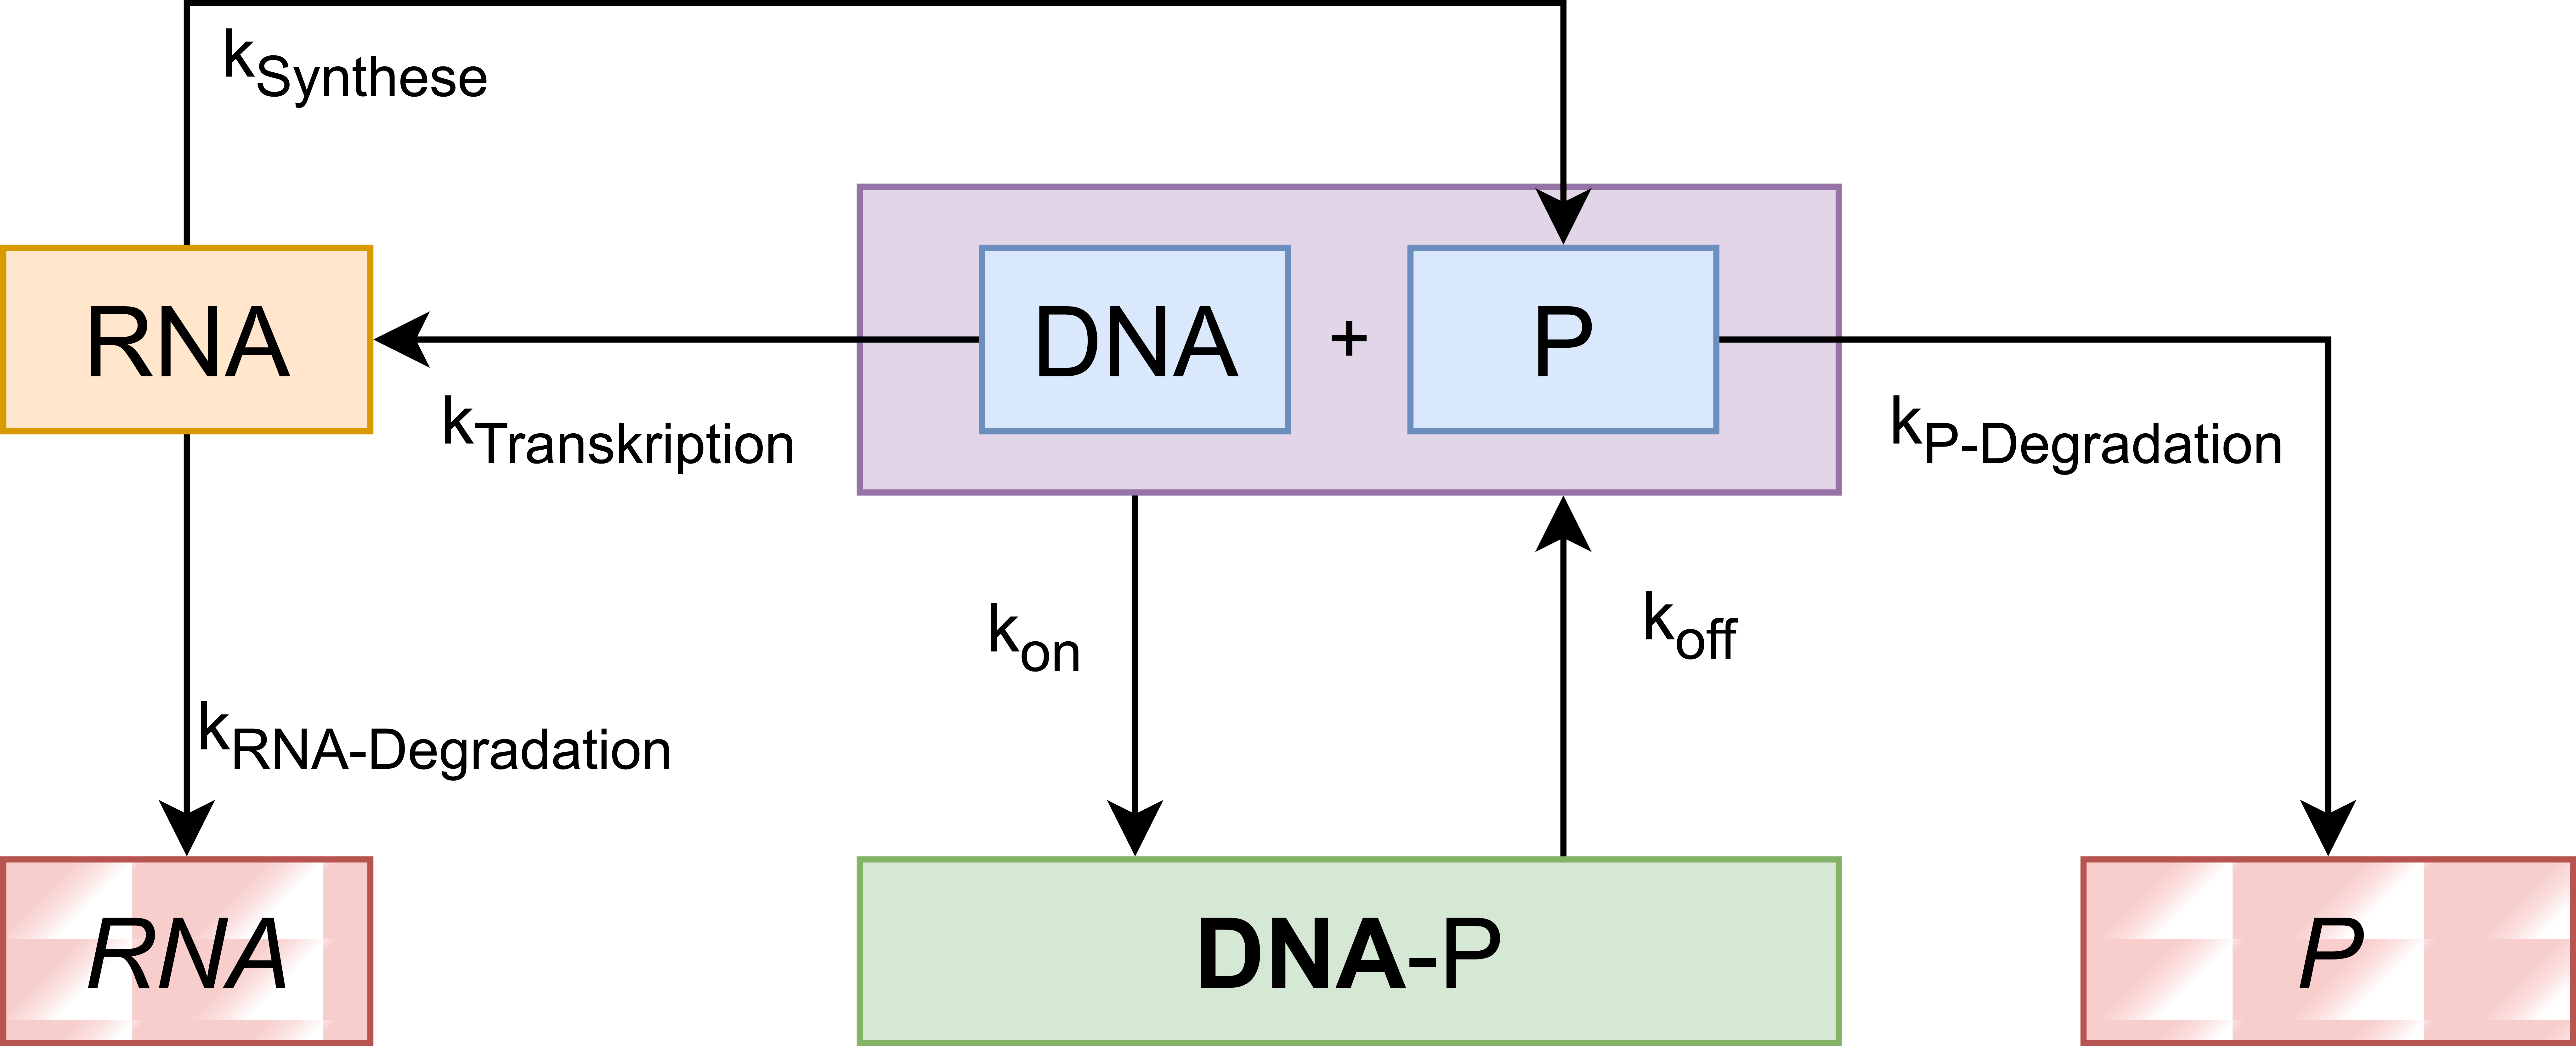
\includegraphics[width=\textwidth]{images/negative_autoregulation_overview.png}

%@Xaver
%\note{Mit Overview neuen Kontext einleiten}
\end{frame}

\begin{frame}{Mathematische Modellierung}
\begin{columns}
    \column{.5\textwidth}
    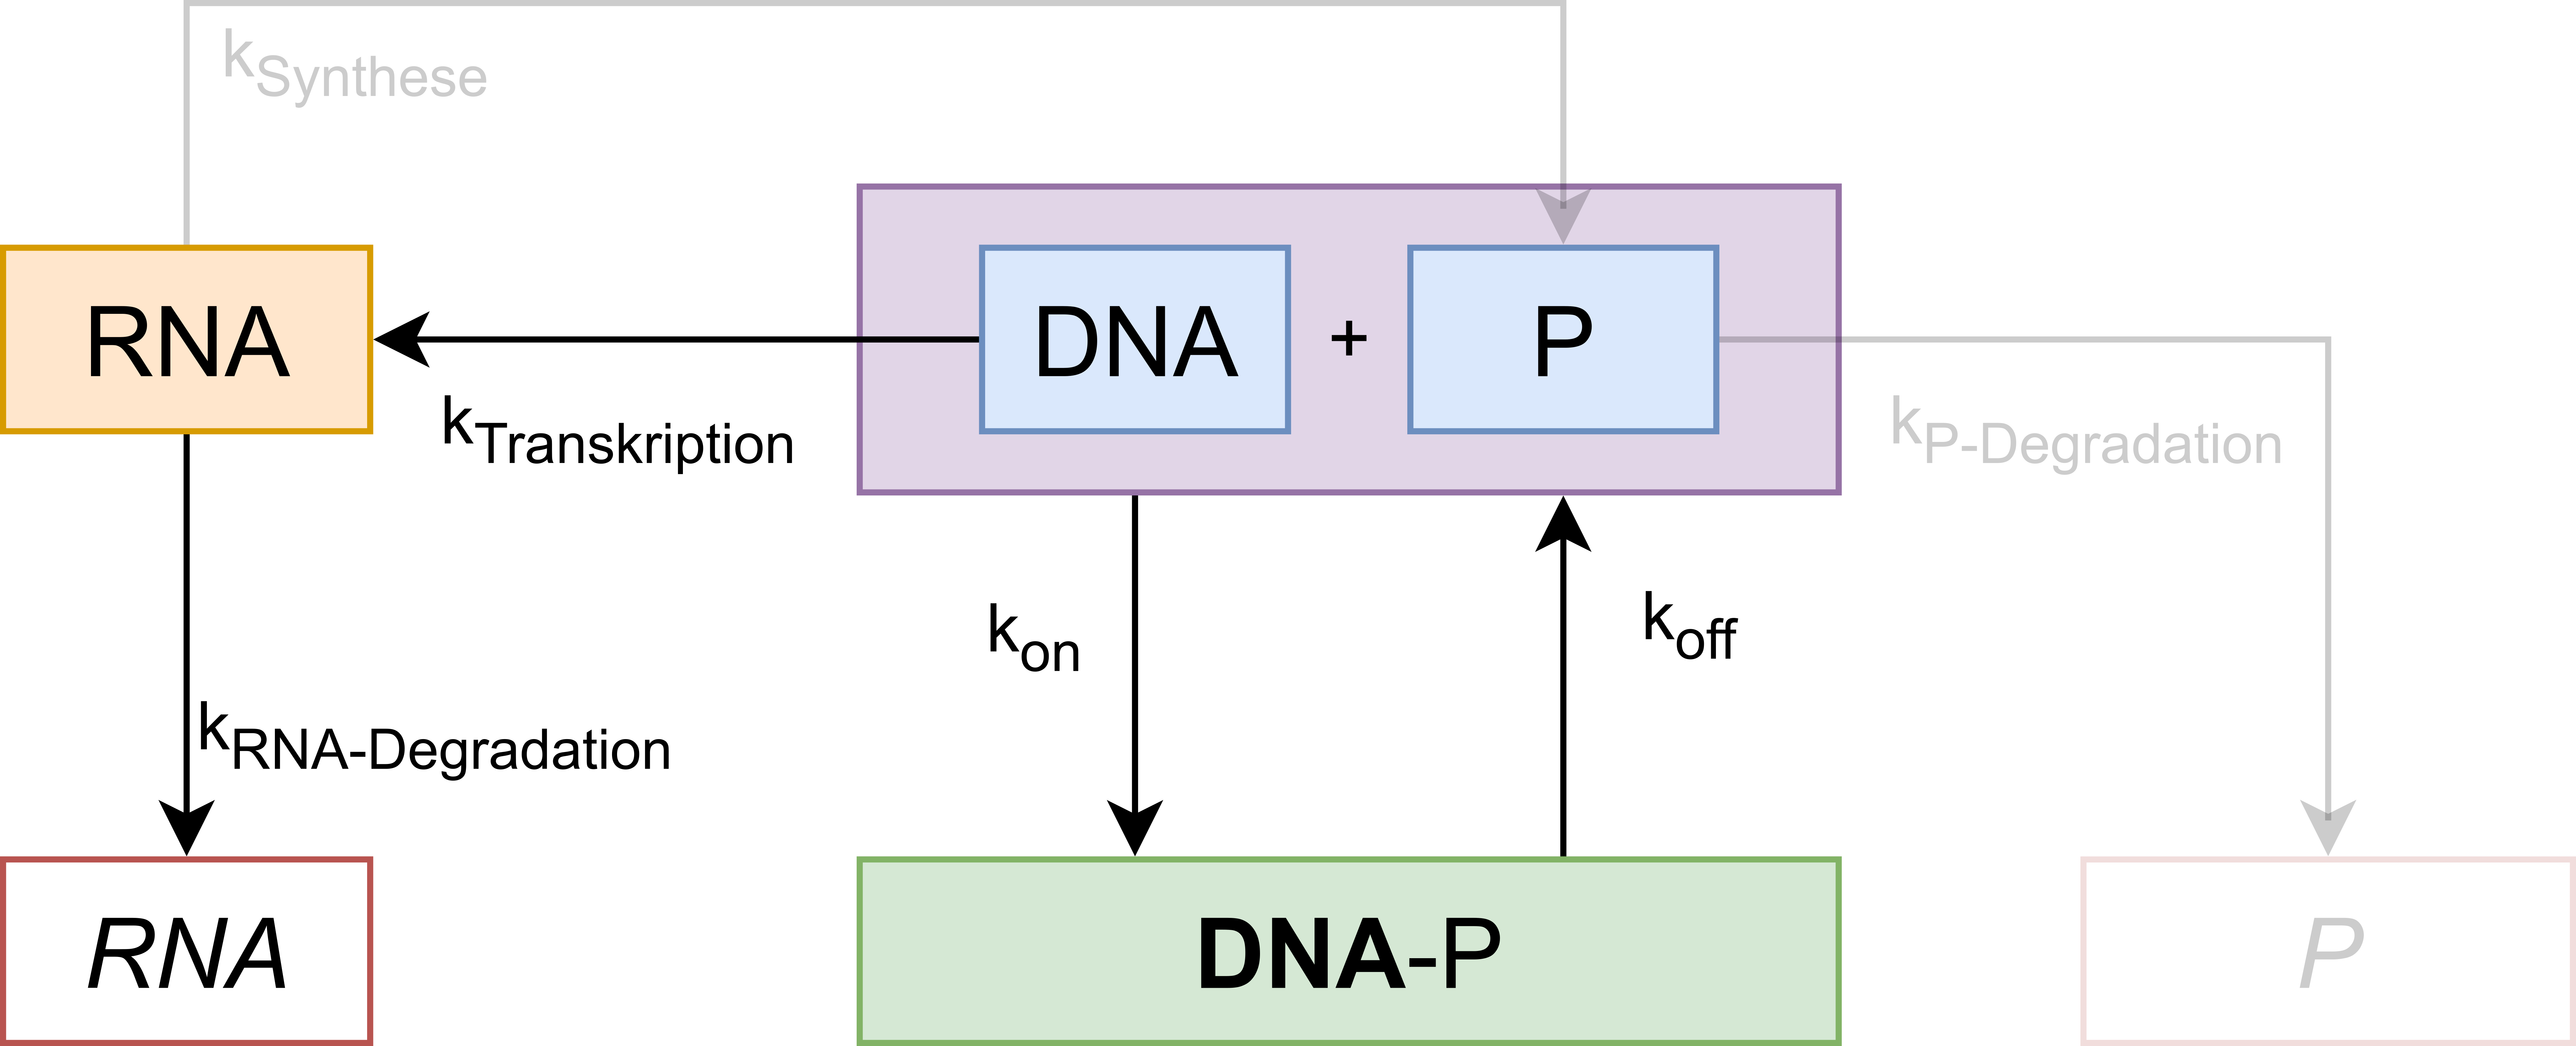
\includegraphics[width=\textwidth]{images/negative_autoregulation_RNA.png}
    \column{.5\textwidth}
    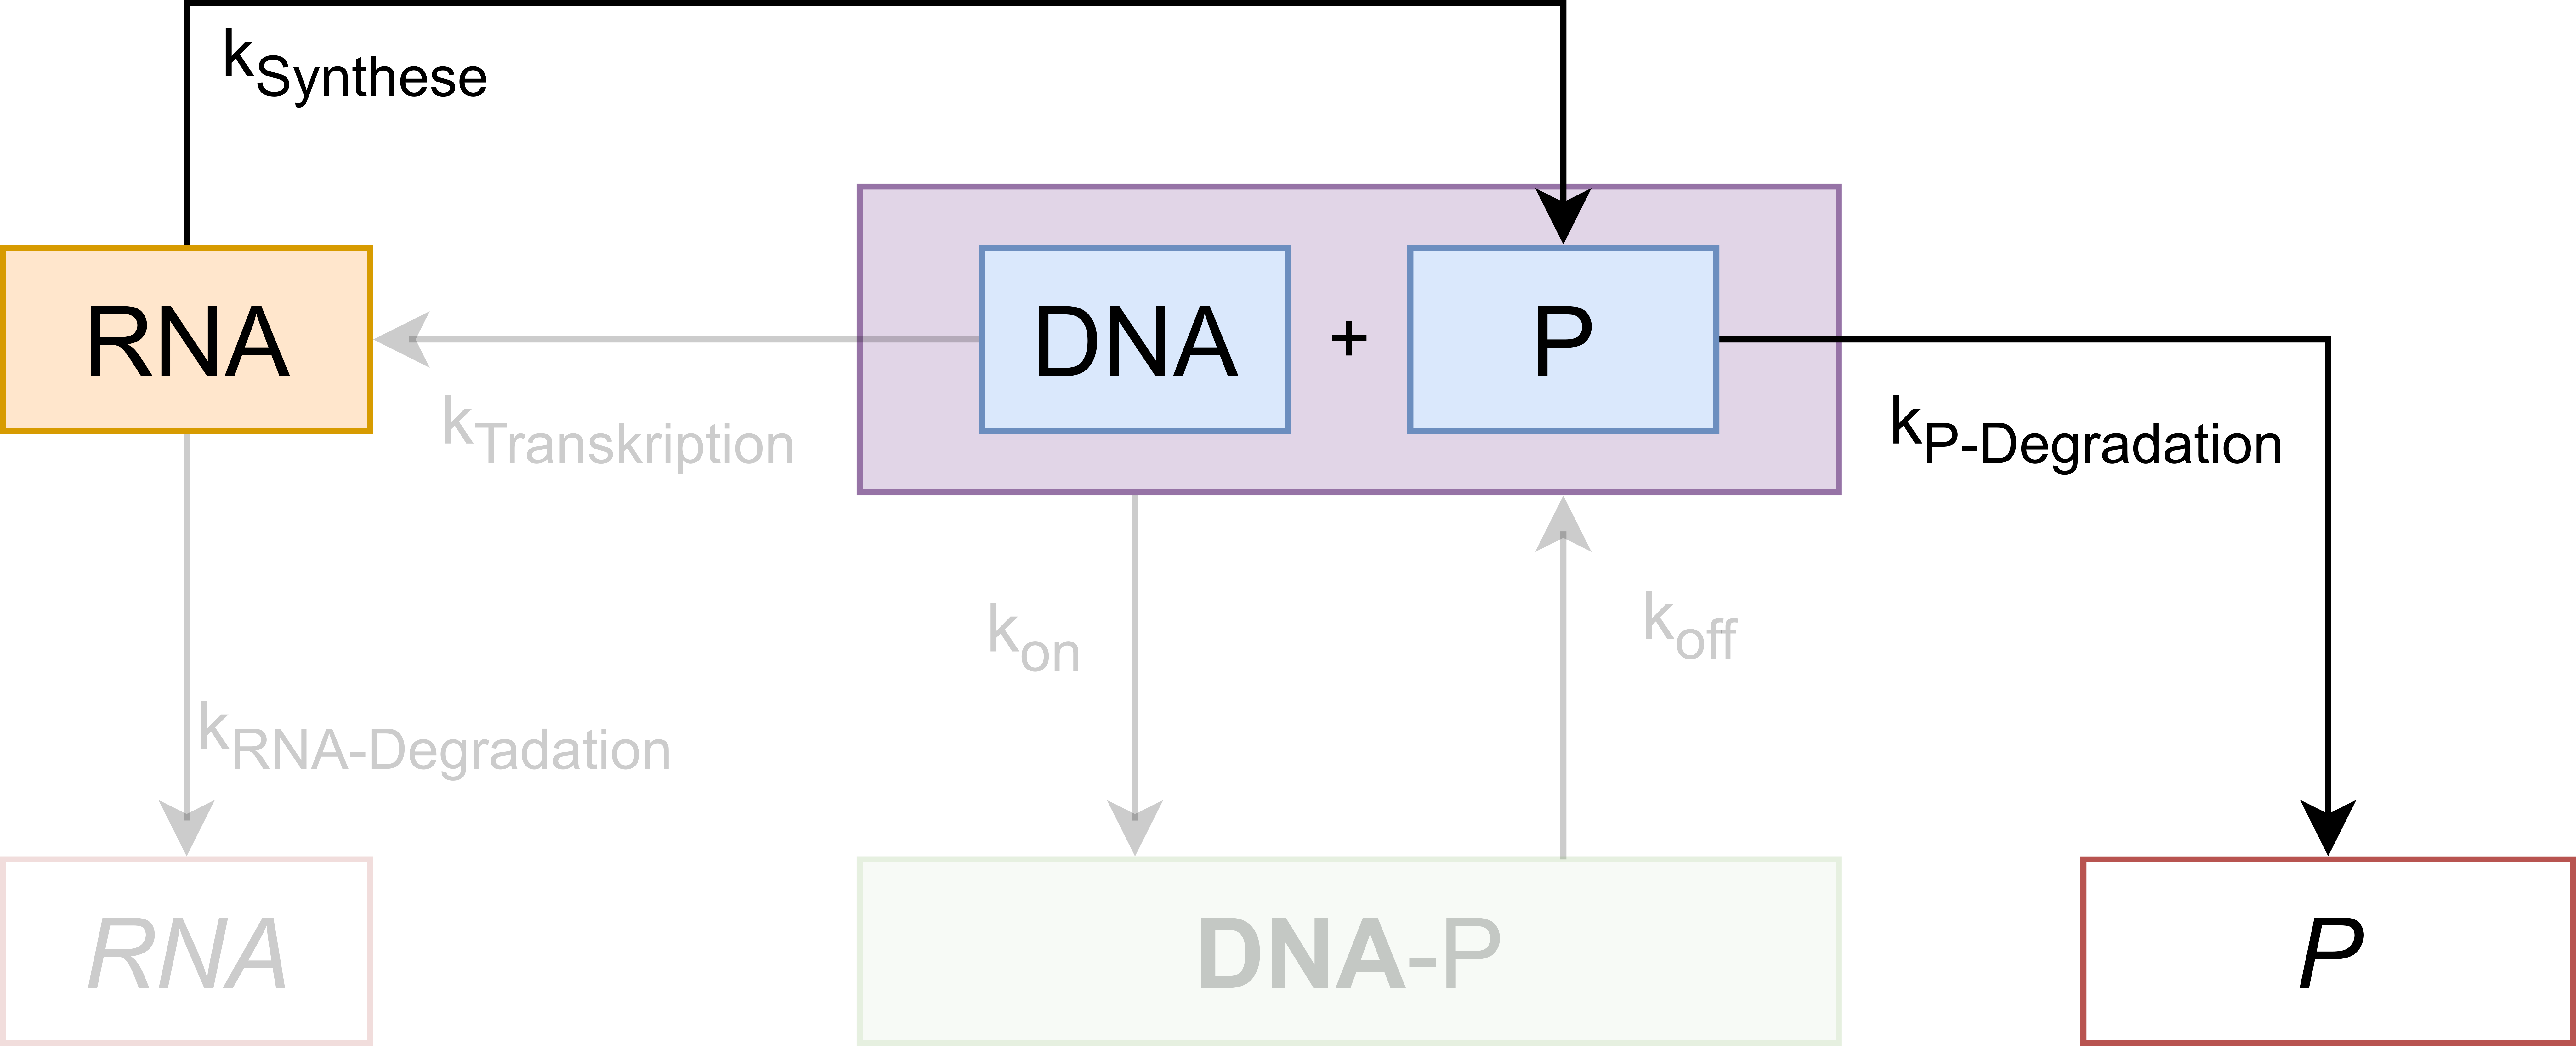
\includegraphics[width=\textwidth]{images/negative_autoregulation_P.png}
\end{columns}
\pause
\vspace{24pt}
\begin{columns}
    \column{.5\textwidth}
    \[\frac{d[\text{RNA}]}{dt}=\text{RNA}_{\text{Synthese}}-\text{RNA}_{\text{Degradation}}\]
    \column{.5\textwidth}
    \[\frac{d[\text{P}]}{dt}=\text{P}_{\text{Synthese}}-\text{P}_{\text{Degradation}}\]
\end{columns}

\end{frame}

\begin{frame}{Mathematische Modellierung mRNA}
    
    \begin{columns}
        \column{0.5\textwidth}
            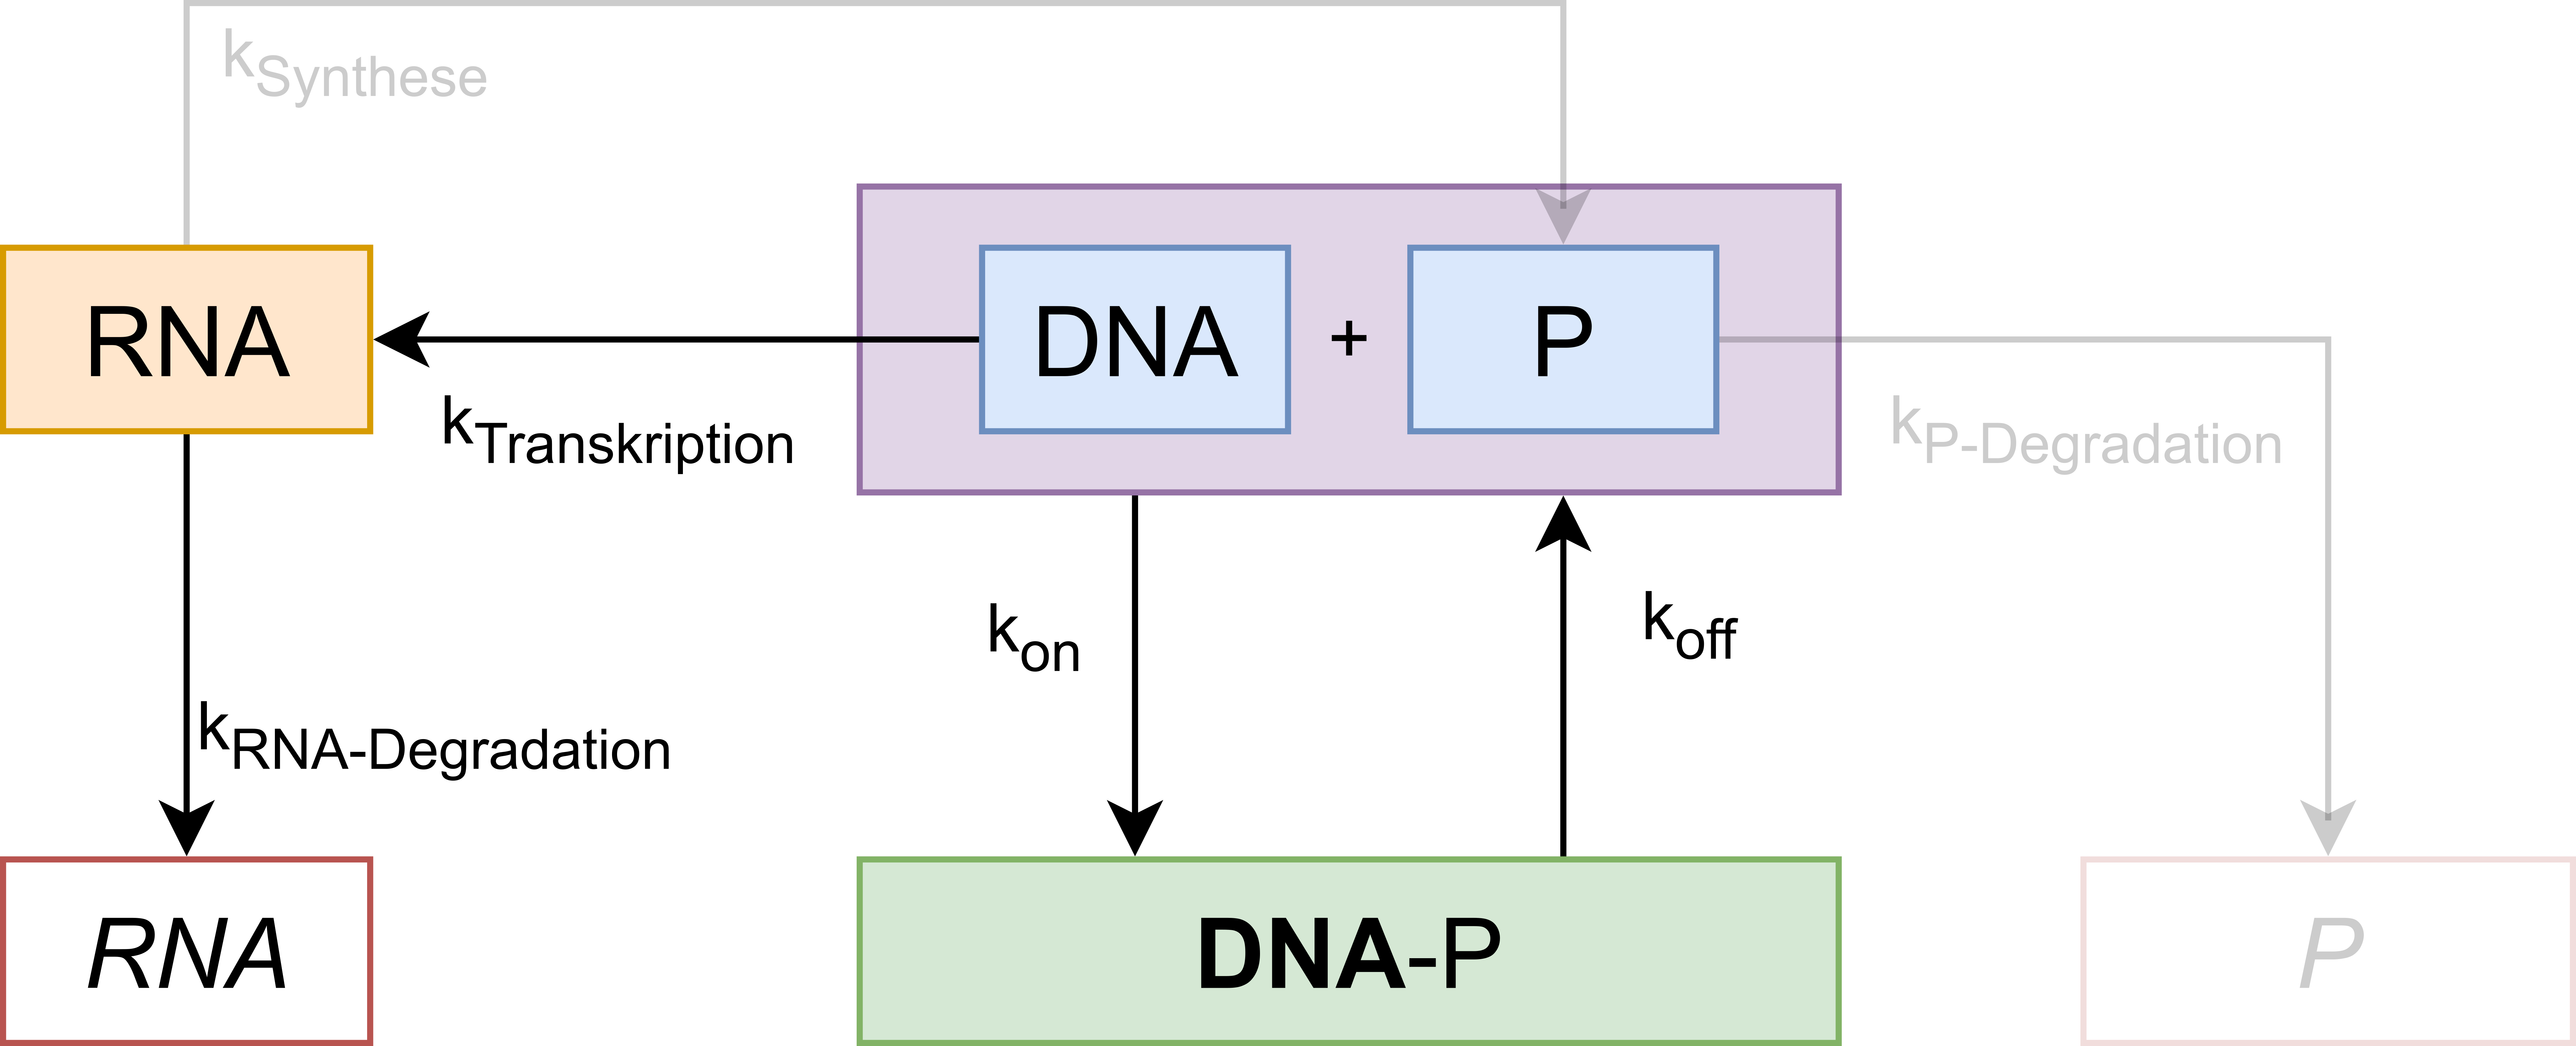
\includegraphics[width=\textwidth]{images/negative_autoregulation_RNA.png}
        \column{0.5\textwidth}

        % pause does not work with the align environment
        \begin{align*}
            \action<+->{\frac{d[\text{RNA}]}{dt}&=\text{RNA}_{\text{Transkription}}-\text{RNA}_{\text{Degradation}}\\[2em]}
            \action<+->{\text{RNA}_{\text{Transkription}}&=}\only<+>{k_\text{t}\cdot [\text{DNA}]}\only<+->{k_{\text{t}} \cdot [\text{DNA}_\text{Total}]  \cdot \frac{K}{K+[\text{P}]}}\\
            \action<+->{\text{RNA}_{\text{Degradation}}&=}\action<+->{k_{dr} \cdot [\text{RNA}]}
        \end{align*}
    \end{columns}

    \vspace{3em}
    \[\action<+->{\frac{d[\text{RNA}]}{dt}=\action<+->{\underbrace{k_{\text{t}} \cdot [\text{DNA}_\text{Total}]}_{v_\text{max}} \cdot \frac{K}{K+[\text{P}]}-k_{dr} \cdot [\text{RNA}]}}\]
\end{frame}

\begin{frame}{Mathematische Modellierung Protein}
    \begin{columns}
        \column{0.5\textwidth}
            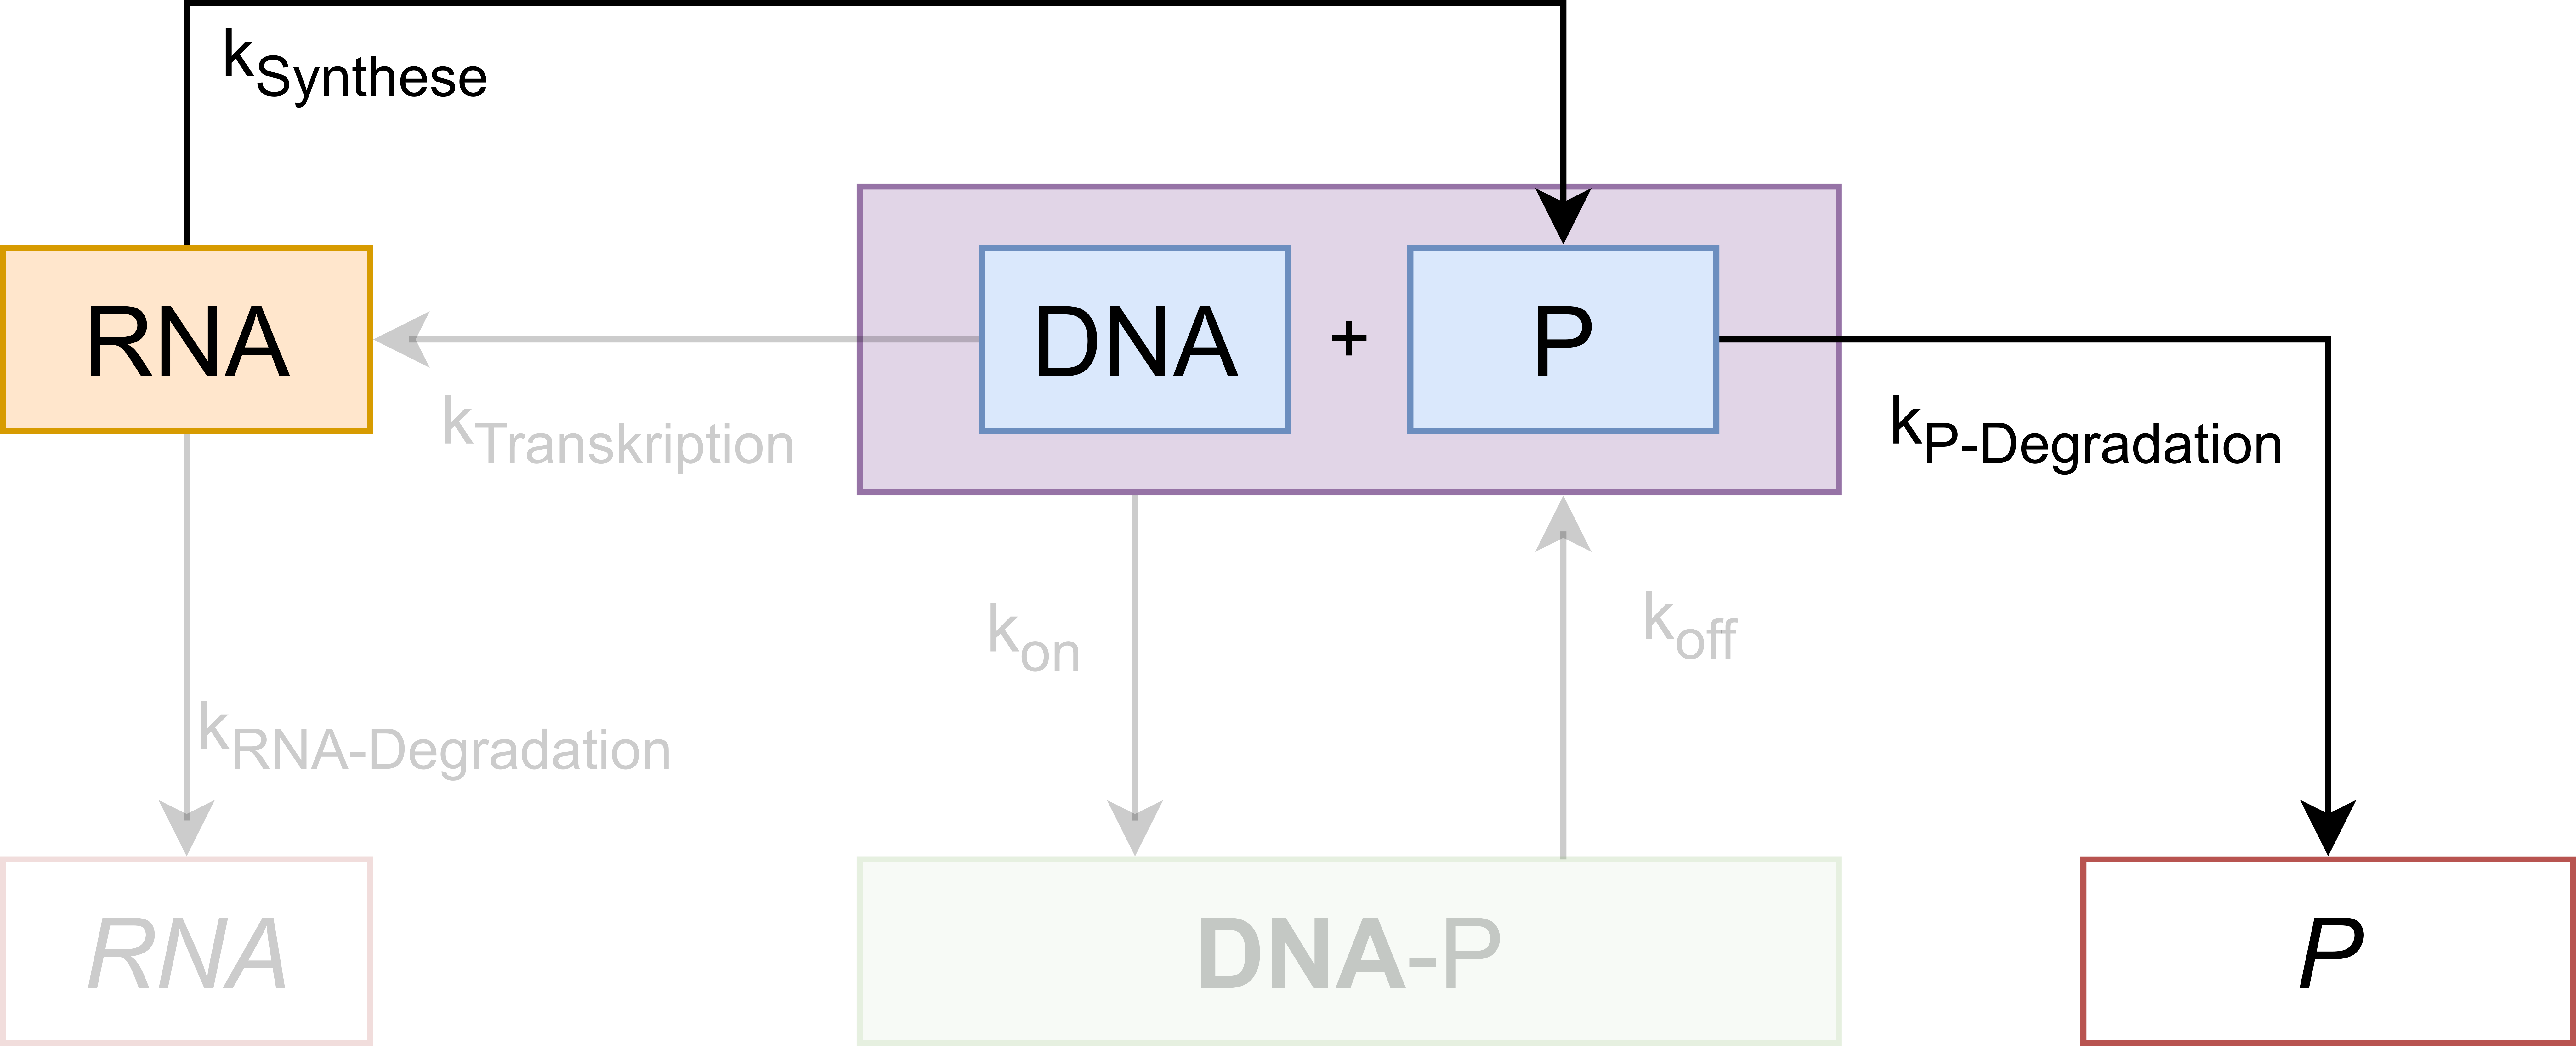
\includegraphics[width=\textwidth]{images/negative_autoregulation_P.png}
        \column{0.5\textwidth}

        \begin{align*}
            \action<+->{\frac{d[\text{P}]}{dt}&=\text{P}_{\text{Synthese}}-\text{P}_{\text{Degradation}}\\[2em]}
            \action<+->{\text{P}_{\text{Synthese}}&=\action<+->{k_s\cdot [\text{RNA}]}\\}
            \action<+->{\text{P}_{\text{Degradation}}&=\action<+->{k_{dp}\cdot [\text{P}]}}
        \end{align*}
    \end{columns}

    \vspace{3em}
    \[\action<+->{\frac{d[\text{P}]}{dt}=\action<+->{k_s\cdot[\text{RNA}]-k_{dp}\cdot[\text{P}]}}\]
\end{frame}

\begin{frame}{Mathematische Modellierung}
    \begin{columns}
        \column{.3\textwidth}
        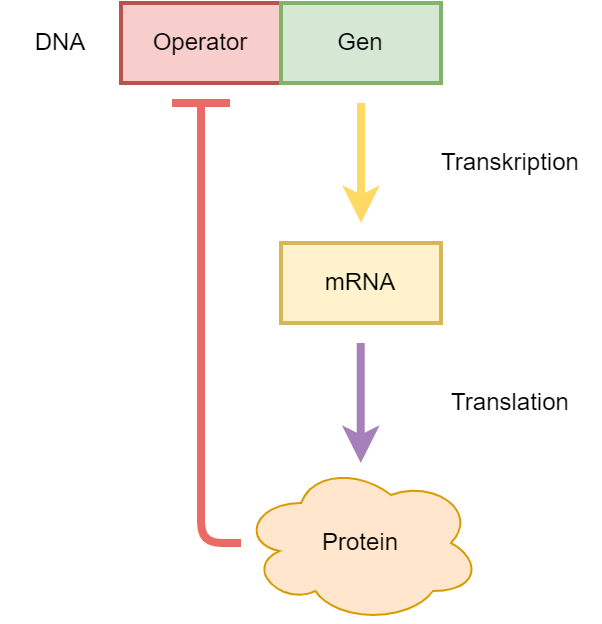
\includegraphics[width=\textwidth]{images/repression.png}
        \column{.7\textwidth}
        \begin{align*}
            \colorbox[HTML]{FFD966}{$\dfrac{d[\text{RNA}]}{dt}$}&=v_{\text{max}}\cdot\frac{K}{K+[\text{P}]}-[\text{RNA}] \cdot k_{dr}\\[16pt]
            \colorbox[HTML]{A680B8}{$\dfrac{d[\text{P}]}{dt}$}&=k_s\cdot[\text{RNA}]-k_{dp}\cdot[\text{P}]
        \end{align*}
    \end{columns}
\end{frame}

\begin{frame}[t]{Stationäre Lösung mRNA herleiten}
    \begin{columns}[t]
        \column{.5\textwidth}
            \[\frac{d[\text{RNA}]}{dt}=v_{\text{max}}\cdot\frac{K}{K+[\text{P}]}-[\text{RNA}] \cdot k_{dr}\]
        \column{.5\textwidth}
            \[\frac{d[\text{P}]}{dt}= k_s\cdot[\text{RNA}]-k_{dp}\cdot[\text{P}]\]
    \end{columns}
    \vspace{20pt}
    \pause
    \begin{columns}[t]
        \column{.5\textwidth}
            \[\]
        \column{.5\textwidth}
            \[0=v_{\text{max}}\cdot\frac{K}{K+[\text{P}]}-[\text{RNA}] \cdot k_{dr}\]
    \end{columns}
    \pause
    \begin{columns}[t]
        \column{.5\textwidth}
            \begin{align*}
                0&= k_s\cdot[\text{RNA}]-k_{dp}\cdot[\text{P}] \\
                \Rightarrow [\text{RNA}]&=\frac{k_{dp} \cdot [\text{P}]}{k_s}
            \end{align*}
            %\[\Downarrow\]
            %\[[\text{RNA}]=\frac{k_{dp} \cdot [P]}{k_s}\]
        \column{.5\textwidth}
            \[\Rightarrow 0=v_{\text{max}}\cdot\frac{K}{K+[\text{P}]}-{\frac{k_{dp} \cdot [\text{P}]}{k_s}} \cdot k_{dr}\]
    \end{columns}
    
%@Xaver
\end{frame}

\begin{frame}{Konstanten}
    @Xaver
    \emph{Stationäre Lösung numerisch lösen}
\end{frame}

\begin{frame}{Stationäre Lösung Protein}
@Xaver
Nur eines der beiden herleiten
\end{frame}

\begin{frame}{Numerische Lösung mit Matlab}
@Mario
\end{frame}

\begin{frame}{Biologische Bedeutung}
\end{frame}

\begin{frame}{Vergleich mit positiver Rückkopplung}
@Mario matlab Lösung zeigen
\end{frame}

\begin{frame}{Vereinfachungen}
    \begin{itemize}
        \item Sofortige Einstellung GGW DNA
        \item kein CAP
        \item Lactose $\rightleftharpoons$ Allolactose
        \item "Lactase"
        \item Glucose Repression
        \item 0 Lactose Leckströme
        \item Lactose Uptake
        \item Kooperative Bindung LacI
        \item Konstanter Abbau Protein/mRNA
    \end{itemize}
\end{frame}

\end{document}